
\paragraph{Monkeys exhibit hallmarks of color category behavior}

The animals examined show a hallmark of color categorization behavior: memory biases towards a set of particular points in a perceptually uniform colorspace.
In \autoref{fig:BiasCurves} it can be seen that the confidence intervals deviate substantially from the dashed zero line, with the attractor points being found where the black line crosses the zero line from positive to negative (going counter-clockwise) and the repeller points are found where the line crosses from negative to positive. 

\begin{figure}
\includesvg[inkscapelatex=false, width=\textwidth]{../../Figures/F3_BiasCurves_v1.svg}
\caption{\textbf{Bias as a function of hue.} 
\emph{Black dotted line:} The zero lines where responses would fall if there were no biases.
\emph{Black line:} Bias as a function of hue for monkeys M1, M2, M3 and M4, smoothed with a moving average filter of 5 cues. 
\emph{Gray filled:} confidence intervals for the line, computed through bootstrapping . 
\emph{Colored radiating line:} Median attractor point from bootstrap procedure.
\emph{Colored wedge:} Confidence intervals for the 2.5\% and 97.5\% percentiles for the bootstrapped attractor points.
See Methods for further details.} % CIELUV. Hues approximate.
\label{fig:BiasCurves}
\end{figure}


\paragraph{Shared color categories across monkeys}

We see that all tested monkeys share two common attractor points, which we interpret as evidence of two shared color categories: a warm/orange-ish category (between 0$^\circ$ and 45$^\circ$), and a cool/blue-ish category (between 180$^\circ$ and 225$^\circ$).
In the absence of language, we can infer that these shared categories arise either due to innate biological factors, environmental factors such as the distribution of colors in the terrestrial environment, or a combination of the two.
These categories align well with the daylight locus, and also the object/category distinction previously identified.

\paragraph{Individual differences between monkeys}

In one animal we see evidence of additional categories: strong evidence for a greenish category and weak evidence for a purple category.


\paragraph{Controls for non-uniformity of colorspace}

We (hopefully will) disambiguate biases that arise from residual non-uniformity in the colorspace, and those that arise from memory biases.

It is plausible that there are non-uniformities in CIELUV that may result in our nominally iso-saturated colors actually appearing to have variable saturation. This would be a concern, as it would be a reasonable prediction that higher saturation colors would be more salient, and thus more likely to be selected as responses. In a control experiment we see no (or very little) bias towards higher saturation colors.

% Results table?


\paragraph{Learning rates/DKL}
\paragraph{Limitations of colorspace}
\paragraph{Comparison with humans} % /Panichello
\paragraph{Independent verification of found categories}

\begin{figure}
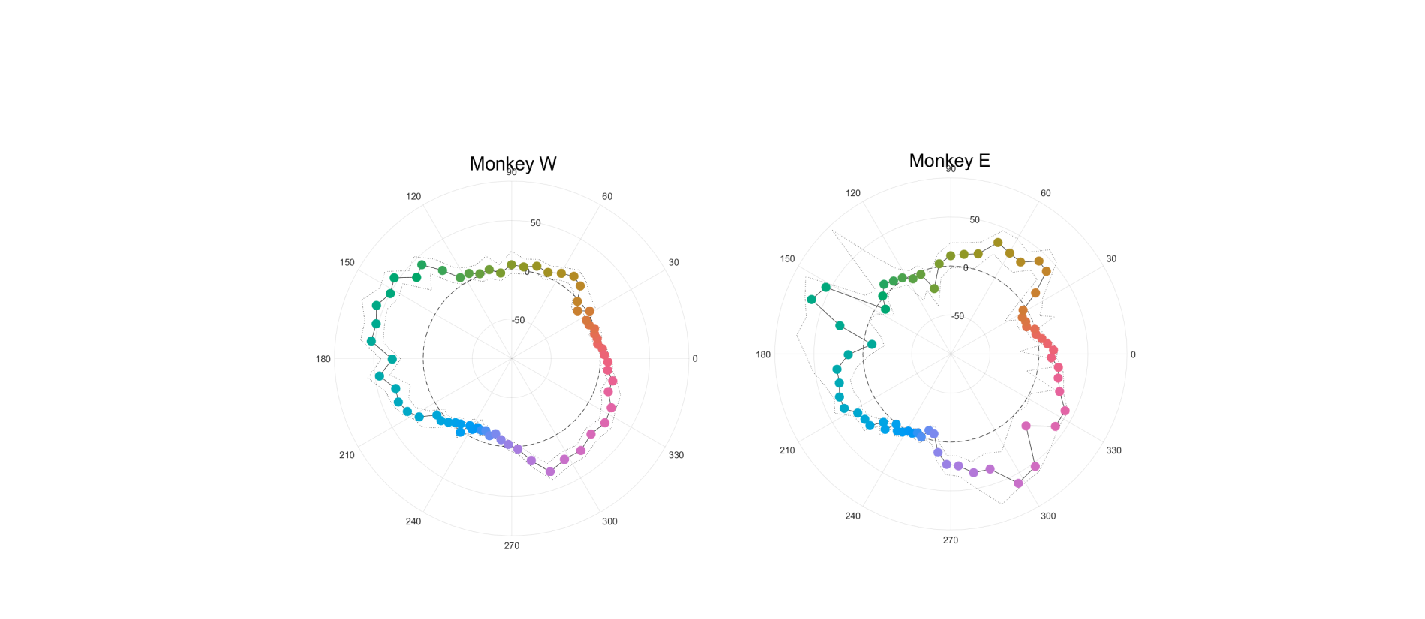
\includegraphics[width=\textwidth]{../../Figures/Old/panichellobias.pdf}
\caption{Bias as a function of hue, for Panichello monkeys} 
\end{figure}


